\subsection{Type checking}
\begin{figure*}
\scriptsize{
\medskip
%%%%%%%%%%%%%%%%%%%%
$
\inferrule
{
}
{
\lins;\ABlockAny \vdash \skipstmt : \lins
}
\;(\textsc{Skip})
$
\medskip
%%%%%%%%%%%%%%%%%%%%
$
\inferrule
{
}
{
\lins;\ABlockOutside \vdash \assert{\locExpr} : \lins
}
\;(\textsc{Assert})
$
\medskip
%%%%%%%%%%%%%%%%%%%%
$
\inferrule
{
\lins_y \subseteq \lins
}
{
\lins;\ABlockOutside \vdash \yield{e,\lins_y} : \lins
}
\;(\textsc{Yield})
$
\medskip
%%%%%%%%%%%%%%%%%%%%
$
\inferrule
{
\ProcLins(A) = (\lins,\lins')
}
{
\lins;\ABlockInside \vdash \call{A} : \lins'
}
\;(\textsc{Atomic})
$
\medskip
%%%%%%%%%%%%%%%%%%%%
$
\inferrule
{
\ProcLins(P) = (\lins,\lins') \\
}
{
\lins;\ABlockOutside \vdash \call{P} : \lins'
}
\;(\textsc{Proc})
$
\medskip
%%%%%%%%%%%%%%%%%%%%
$
\inferrule
{
\lins_G \subseteq \Global \\
\lins \cup \lins_P \cup \lins_P' \subseteq \ThreadLocal \\
\ProcLins(P) = ((\lins_G,\lins_P),(\lins_G,\lins_P')) \\
}
{
\lins_G,\lins,\lins_P;\ABlockOutside \vdash \async{P} : \lins_G,\lins
}
\;(\textsc{Async})
$
\medskip
%%%%%%%%%%%%%%%%%%%%
$
\inferrule
{
\lins;\ABlockInside \vdash \stmt : \lins' \\
\lins_a \subseteq \lins
}
{
\lins;\ABlockOutside \vdash \ablock{e,\lins_a}{\stmt} : \lins'
}
\;(\textsc{Ablock})
$
\medskip
%%%%%%%%%%%%%%%%%%%%
$
\inferrule
{
\lins;\ABlockAny \vdash \StmtStack : \lins'
}
{
\lins;\ABlockAny \vdash (\varsL,\StmtStack) : \lins'
}
\;(\textsc{Stack})
$
\medskip
%%%%%%%%%%%%%%%%%%%%
$
\inferrule
{
\lins;\ABlockAny \vdash \StmtStack : \lins' \\
\lins';\ABlockAny \vdash \stmt : \lins''
}
{
\lins;\ABlockAny \vdash \StmtStack;\stmt : \lins''
}
\;(\textsc{Seq})
$
\medskip
%%%%%%%%%%%%%%%%%%%%
$
\inferrule
{
\lins;\ABlockAny \vdash s_1 : \lins' \\
\lins;\ABlockAny \vdash s_2 : \lins'
}
{
\lins;\ABlockAny \vdash \ite{\locExpr}{s_1}{s_2} : \lins'
}
\;(\textsc{Ite})
$
\medskip
%%%%%%%%%%%%%%%%%%%%
$
\inferrule
{
\lins;\ABlockAny \vdash s : \lins
}
{
\lins;\ABlockAny \vdash \while{e,\alpha}{\locExpr}{s} : \lins
}
\;(\textsc{While})
$
\medskip
%%%%%%%%%%%%%%%%%%%%
$
\inferrule
{
\ProcLins(P) = (\lins,\lins') \\
\procs(P) = (\phi, \mods, \psi, \stmt) \\
\lins;\ABlockOutside \vdash \stmt : \lins'
}
{
\vdash P
}
\;(\textsc{Procedure})
$
\medskip
%%%%%%%%%%%%%%%%%%%%
$
\inferrule
{
T = (\varsTL, (\varsL, \StmtStack)) \\
\lins;\ABlockOutside \vdash \StmtStack : \lins'
}
{
\lins \vdash T
}
\;(\textsc{Thread})
$
\medskip
%%%%%%%%%%%%%%%%%%%%
$
\inferrule
{
\ProcLins(A) = (\lins,\lins') \\
\lins \cap \Global = \lins' \cap \Global \\
\actions(A) = (\rho, \alpha, m) \\\\
\forall (\sigma,\sigma') \in \alpha.
  \disjoint(\{\sigma(x) \mid x \in \lins\}) \wedge
  \disjoint(\{\sigma'(x) \mid x \in \lins'\}) \\
\forall (\sigma,\sigma') \in \alpha.
  \bigcup\{\sigma'(x) \mid x \in \lins'\} \subseteq \bigcup\{\sigma(x) \mid x \in \lins\}
}
{
\vdash A
}
\;(\textsc{Action})
$
\medskip
%%%%%%%%%%%%%%%%%%%%
$
\inferrule
{
\forall P \in \ProcName. \vdash P \\
\forall A \in \ActionName. \vdash A \\
\lins_G \subseteq \Global \\
\forall 1 \le i \le n. (\lins_G,\lins_i \vdash T_i) \\
\forall 1 \le i \le n. (\lins_i \subseteq \ThreadLocal) \\
\forall 1 \le i \le n. (T_i = (\varsTL_i, \ldots)) \\
\disjoint(\{\varsG(x) \mid x \in \lins_G\} \cup
  \{\varsTL_i(x) \mid 1 \le i \le n, x \in \lins_i\})
}
{
\vdash (\procs, \actions, \ProcLins, \varsG, T_1 \ldots T_n)
}
\;(\textsc{Program})
$
\medskip
%%%%%%%%%%%%%%%%%%%%
}
\caption{Type checking rules}
\label{fig:type-checking}
\end{figure*}

\subsection{Safety}
\begin{figure}
\scriptsize{
\medskip
%%%%%%%%%%%%%%%%%%%%
$
\inferrule
{
}
{\procs;\actions;\RefinementAny;\{\} \jp \FH{\phi}{\skipstmt}{\phi}}
\;(\textsc{Skip})
$
\medskip\\
%%%%%%%%%%%%%%%%%%%%
$
\inferrule
{
}
{\procs;\actions;\RefinementOutside;\{\} \jp \FH{\phi}{\assert{\locExpr}}{\phi}}
\;(\textsc{Assert1})
$
\medskip
%%%%%%%%%%%%%%%%%%%%
$
\inferrule
{
}
{\procs;\actions;\RefinementInside;\{\} \jp \FH{\phi \wedge \locExpr}{\assert{\locExpr}}{\phi}}
\;(\textsc{Assert2})
$
\medskip
%%%%%%%%%%%%%%%%%%%%
$
\inferrule
{
}
{\procs;\actions;\RefinementAny;\{\} \jp \FH{e}{\yield{e,\lins}}{e}}
\;(\textsc{Yield})
$
\medskip
%%%%%%%%%%%%%%%%%%%%
$
\inferrule
{
\actions(A) = (\rho, \alpha, m) \\ 
\mods \subseteq \ThreadLocal \\
\alpha \Rightarrow \Havoc(\Global \cup \mods \cup \Local) \\
\phi \Rightarrow \rho \\ 
\Unsat{\phi \circ \alpha \circ \neg \psi} \\
}
{\procs;\actions;\RefinementAny;\mods \jp \FH{\phi}{\call{A}}{\psi}}
\;(\textsc{Atomic})
$
\medskip
%%%%%%%%%%%%%%%%%%%%
$
\inferrule
{
\procs(P) = (\phi, \mods, \psi, \stmt) \\ P \not \in \dom(\Refines)
}
{\procs;\actions;\RefinementAny;\mods \jp \FH{\phi}{\call{P}}{\psi}}
\;(\textsc{Proc1})
$
\medskip
%%%%%%%%%%%%%%%%%%%%
$
\inferrule
{
\procs(P) = (\phi, \mods, \psi, \stmt) \\ P \in \dom(\Refines) \\\\ \procs;\actions;\RefinementAny;\mods \jp \FH{\phi}{\call{\Refines(P)}}{\psi}
}
{\procs;\actions;\RefinementAny;\mods \jp \FH{\phi}{\call{P}}{\psi}}
\;(\textsc{Proc2})
$
\medskip
%%%%%%%%%%%%%%%%%%%%
$
\inferrule
{
\procs(P) = (\phi, \mods, \psi, \stmt)
}
{\procs;\actions;\RefinementAny;\{\} \jp \FH{\rho \wedge \phi}{\async{P}}{\rho}}
\;(\textsc{Async})
$
\medskip\\
%%%%%%%%%%%%%%%%%%%%
$
\inferrule
{
\procs;\actions;\RefinementAny;\mods \jp \FH{\phi_1 \wedge e}{s}{\phi_2}
}
{\procs;\actions;\RefinementAny;\mods \jp \FH{\phi_1 \wedge e}{\ablock{e,\lins}{s}}{\phi_2}}
\;(\textsc{Ablock})
$
\medskip
%%%%%%%%%%%%%%%%%%%%
$
\inferrule
{
\procs;\actions;\RefinementAny;\mods_1 \jp \FH{\phi_1}{\StmtStack}{\phi_2} \\ 
\procs;\actions;\RefinementAny;\mods_2 \jp \FH{\phi_2}{s}{\phi_3}
}
{\procs;\actions;\RefinementAny;\mods_1 \cup \mods_2 \jp \FH{\phi_1}{\StmtStack;s}{\phi_3}}
\;(\textsc{Seq})
$
\medskip
%%%%%%%%%%%%%%%%%%%%
$
\inferrule
{
\procs;\actions;\RefinementAny;\mods_1 \jp \FH{e \wedge \phi_1}{s_1}{\phi_2} \\ 
\procs;\actions;\RefinementAny;\mods_2 \jp \FH{\neg e \wedge \phi_1}{s_2}{\phi_2}
}
{\procs;\actions;\RefinementAny;\mods_1 \cup \mods_2 \jp \FH{\phi_1}{\ite{\locExpr}{s_1}{s_2}}{\phi_2}}
\;(\textsc{Ite})
$
\medskip
%%%%%%%%%%%%%%%%%%%%
$
\inferrule
{
\procs;\actions;\RefinementAny;\mods \jp \FH{e \wedge \locExpr}{s}{e}
}
{\procs;\actions;\RefinementAny;\mods \jp \FH{e}{\while{e,\alpha}{\locExpr}{s}}{e \wedge \neg \locExpr}}
\;(\textsc{While})
$
\medskip
%%%%%%%%%%%%%%%%%%%%
$
\inferrule
{
\phi \Rightarrow \phi' \\ \procs;\actions;\RefinementAny;\mods \jp \FH{\phi'}{\StmtStack}{\psi'} \\ \psi' \Rightarrow \psi
}
{\procs;\actions;\RefinementAny;\mods \jp \FH{\phi}{\StmtStack}{\psi}}
\;(\textsc{Weaken})
$
\medskip
%%%%%%%%%%%%%%%%%%%%
$
\inferrule
{
\procs;\actions;\RefinementAny;\mods \jp \FH{\phi}{\StmtStack}{\psi} \\ \accessVars(\rho) \cap \mods = \{\}
}
{\procs;\actions;\RefinementAny;\mods \jp \FH{\rho \wedge \phi}{\StmtStack}{\rho \wedge \psi}}
\;(\textsc{Frame})
$
\medskip
%%%%%%%%%%%%%%%%%%%%
$
\inferrule
{
\procs(P) = (\phi, \mods, \psi, \stmt) \\
\RefinementAny = \RefinementInside \Longleftrightarrow P \in \dom(\Refines) \\\\
\procs;\actions;\RefinementAny;\mods' \jp \FH{\phi}{\stmt}{\psi} \\
\mods' \subseteq \mods
}
{
\procs;\actions;\Refines \jp P
}
\;(\textsc{Procedure})
$
\medskip
%%%%%%%%%%%%%%%%%%%%
$
\inferrule
{
\procs;\actions;\RefinementAny;\mods \jp \FH{\phi'}{\StmtStack}{\psi} \\\\
(\accessVars(\phi) \cup \accessVars(\psi)) \cap \Local = \{\} \\\\
\forall \varsG,\varsTL,\varsL.\ \MakeStore{\varsG}{\varsTL}{\varsL} \in \phi \Rightarrow \MakeStore{\varsG}{\varsTL}{\varsL} \in \phi'
}
{
\procs;\actions;\RefinementAny;\mods \jp \FH{\phi}{(\varsL',\StmtStack)}{\psi}
}
\;(\textsc{Stack})
$
\medskip
%%%%%%%%%%%%%%%%%%%%
$
\inferrule
{
T = (\varsTL, (\varsL, \StmtStack)) \\
\MakeStore{\varsG}{\varsTL}{\varsL} \in \phi \\
\procs;\actions;\RefinementOutside;\mods \jp \FH{\phi}{\StmtStack}{\true}
}
{
\procs;\actions;\varsG \jp T
}
\;(\textsc{Thread})
$
\medskip
%%%%%%%%%%%%%%%%%%%%
$
\inferrule
{
\forall P \in \ProcName.\ \procs;\actions;\Refines \jp P \\\\
\forall 1 \le i \le n.\ \procs;\actions;\varsG \jp T_i
}
{
\Refines \jp (\procs, \actions, \ProcLins, \varsG, T_1 \ldots T_n)
}
\;(\textsc{Program})
$
\medskip
%%%%%%%%%%%%%%%%%%%%
}
\caption{Sequential rules for partial correctness}
\label{fig:sequential-correctness}
\end{figure}

{\bf Non-interference.}
Let $\Prog = (\procs, \actions, \ProcLins, \varsG, \TS)$ be a program
and $\Refines$ be a refinement map.
Let $\Yields(\Prog)$ be the union of the following sets:
\begin{itemize}
\item
$\{(\phi,\lins) \mid \yield{\phi,\lins}~\mathrm{appears~in~\Prog}\}$.
\item
$\{(\phi,\lins) \mid P \in \ProcName \wedge \procs(P) = (\phi, \mods, \psi, \stmt) \wedge \ProcLins(P) = (\lins,\lins')\}$.
\item
$\{(\psi,\lins') \mid P \in \ProcName \wedge \procs(P) = (\phi, \mods, \psi, \stmt) \wedge \ProcLins(P) = (\lins,\lins')\}$.
\end{itemize}
Let $\Ablocks(\Prog,\Refines)$ be the set of atomic blocks in $\Prog$ except those inside the bodies of procedures
in $\dom(\Refines)$.

Let $\FV \subseteq \VarName \setminus \Var$ be a set of fresh variables and $\Lambda$ be a one-one 
substitution function from $\ThreadLocal \cup \Local$ to $\FV$.
Let $\Lambda(\phi)$ represent the result of applying $\Lambda$ to the expression $\phi$.
The program $\Prog$ is interference-free with respect to $\Refines$, denoted by $\InterferenceFree(\Prog,\Refines)$,
if for each predicate ($\phi,\lins_y) \in \Yields(\Prog)$, the following conditions are satisfied:
\begin{enumerate}
\item
For each atomic block $\ablock{e,\lins_a}{s} \in \Ablocks(\Prog,\Refines)$, the judgment
\[
\FH{\Lambda(\phi) \wedge e \wedge \disjoint(\Lambda(\lins_y \setminus \Global) \cup \lins_a)}{s}{\Lambda(\phi)}
\]
holds.
\item
For each $A \in \range(\Refines)$ such that $\actions(A) = (\rho, \alpha, m)$ and $\ProcLins(A) = (\lins_a,\lins'_a)$, 
\[
(\Lambda(\phi) \wedge \rho \wedge \disjoint(\Lambda(\lins_y \setminus \Global) \cup \lins_a)) \circ \alpha \circ \neg\Lambda(\phi)
\]
is unsatisfiable.
\end{enumerate}

\subsection{Refinement}
\begin{figure}
\scriptsize{
\medskip
%%%%%%%%%%%%%%%%%%%%
$
\inferrule
{
}
{\Refines;\actions;P \jr \skipstmt : \false}
\;(\textsc{Skip})
$
\medskip
%%%%%%%%%%%%%%%%%%%%
$
\inferrule
{
}
{\Refines;\actions;P \jr \assert{\locExpr} : \false}
\;(\textsc{Assert})
$
\medskip
%%%%%%%%%%%%%%%%%%%%
$
\inferrule
{
}
{\Refines;\actions;P \jr \yield{e,\lins} : \false}
\;(\textsc{Yield})
$
\medskip
%%%%%%%%%%%%%%%%%%%%
$
\inferrule
{
P' \in \dom(\Refines) \\ \actions(\Refines(P')) = (\rho',\alpha',m) \\\\ \rho' \circ \alpha' \Rightarrow \Havoc(\{\})
}
{\Refines;\actions;P \jr \call{P'} : \false}
\;(\textsc{Call1})
$
\medskip
%%%%%%%%%%%%%%%%%%%%
$
\inferrule
{
P' \in \dom(\Refines) \\ \actions(\Refines(P)) = (\rho,\alpha,m) \\ 
\actions(\Refines(P')) = (\rho',\alpha',m) \\ \rho' \circ \alpha' \Rightarrow \exists \mathit{old}(\Local), \Local.\ \alpha
}
{\Refines;\actions;P \jr \call{P'} : \true}
\;(\textsc{Call2})
$
\medskip
%%%%%%%%%%%%%%%%%%%%
$
\inferrule
{
P' \in \dom(\Refines) \\ \actions(\Refines(P')) = (\rho',\alpha',m) \\ \rho' \circ \alpha' \Rightarrow \Havoc(\{\})
}
{\Refines;\actions;P \jr \async{P'} : \false}
\;(\textsc{Async})
$
\medskip
%%%%%%%%%%%%%%%%%%%%
$
\inferrule
{
\actions \vdash s \preceq \mathit{old}(e) \Rightarrow \Havoc(L)
}
{\Refines;\actions;P \jr \ablock{e,\lins}{s} : \false}
\;(\textsc{Ablock1})
$
\medskip
%%%%%%%%%%%%%%%%%%%%
$
\inferrule
{
\actions(\Refines(P)) = (\rho,\alpha,m) \\\\
\actions \vdash s \preceq \mathit{old}(e) \Rightarrow  \exists \mathit{old}(\Local), \Local.\ \alpha
}
{\Refines;\actions;P \jr \ablock{e,\lins}{s} : \true}
\;(\textsc{Ablock2})
$
\medskip
%%%%%%%%%%%%%%%%%%%%
$
\inferrule
{
\Refines;\actions;P \jr s_1 : b_1 \\ \Refines;\actions;P \jr s_2 : b_2 \\ \neg(b_1 \wedge b_2)
}
{\Refines;\actions;P \jr s_1;s_2 : b_1 \vee b_2}
\;(\textsc{Seq})
$
\medskip
%%%%%%%%%%%%%%%%%%%%
$
\inferrule
{
\Refines;\actions;P \jr s_1 : b \\ \Refines;\actions;P \jr s_2 : b
}
{\Refines;\actions;P \jr \ite{\locExpr}{s_1}{s_2} : b}
\;(\textsc{Ite})
$
\medskip
%%%%%%%%%%%%%%%%%%%%
$
\inferrule
{
\Refines;\actions;P \jr s : \false
}
{\Refines;\actions;P \jr \while{e,\alpha}{\locExpr}{s} : \false}
\;(\textsc{While})
$
\medskip
%%%%%%%%%%%%%%%%%%%%
$
\inferrule
{
\procs(P) = (\phi, \mods, \psi, \stmt) \\\\
\forall P \in \dom(\Refines).\ \Refines;\actions;P \jr \stmt : \true
}
{
\Refines \jr (\procs, \actions, \ProcLins, \varsG, T_1 \ldots T_n)
}
\;(\textsc{Program})
$
\medskip
%%%%%%%%%%%%%%%%%%%%
}
\caption{Refinement rules}
\label{fig:refinement}
\end{figure}

\begin{figure}
\scriptsize{
\medskip
%%%%%%%%%%%%%%%%%%%%
$
\inferrule
{
}
{\actions \vdash \skipstmt \preceq \Havoc(\{\})}
\;(\textsc{Skip})
$
\medskip
%%%%%%%%%%%%%%%%%%%%
$
\inferrule
{
}
{\actions \vdash \assert{\locExpr} \preceq \Havoc(\{\})}
\;(\textsc{Assert})
$
\medskip
%%%%%%%%%%%%%%%%%%%%
$
\inferrule
{
}
{\actions \vdash \yield{e,\lins} \preceq \false}
\;(\textsc{Yield})
$
\medskip
%%%%%%%%%%%%%%%%%%%%
$
\inferrule
{
\actions(A) = (\rho, \alpha, m) 
}
{\actions \vdash \call{A} \preceq \alpha}
\;(\textsc{Atomic})
$
\medskip
%%%%%%%%%%%%%%%%%%%%
$
\inferrule
{
}
{\actions \vdash \call{P} \preceq \false}
\;(\textsc{Call})
$
\medskip
%%%%%%%%%%%%%%%%%%%%
$
\inferrule
{
}
{\actions \vdash \async{P} \preceq \Havoc(\{\})}
\;(\textsc{Async})
$
\medskip
%%%%%%%%%%%%%%%%%%%%
$
\inferrule
{
s \preceq \alpha
}
{\actions \vdash \ablock{e,\lins}{s} \preceq \alpha}
\;(\textsc{Ablock})
$
\medskip
%%%%%%%%%%%%%%%%%%%%
$
\inferrule
{
\actions \vdash s_1 \preceq \alpha_1 \\\\ \actions \vdash s_2 \preceq \alpha_2
}
{\actions \vdash s_1;s_2 \preceq \alpha_1 \circ \alpha_2}
\;(\textsc{Seq})
$
\medskip
%%%%%%%%%%%%%%%%%%%%
$
\inferrule
{
\actions \vdash s_1 \preceq \alpha_1 \\ \actions \vdash s_2 \preceq \alpha_2
}
{\actions \vdash \ite{\locExpr}{s_1}{s_2} \preceq (\locExpr \circ \alpha_1) \vee (\neg \locExpr \circ \alpha_2)}
\;(\textsc{Ite})
$
\medskip
%%%%%%%%%%%%%%%%%%%%
$
\inferrule
{
\actions \vdash s \preceq \beta \\ \neg \locExpr \circ \Havoc(\{\}) \Rightarrow \alpha \\ \beta \circ \alpha \Rightarrow \alpha 
}
{\actions \vdash \while{e,\alpha}{\locExpr}{s} \preceq e \circ \alpha \circ \neg \locExpr}
\;(\textsc{While})
$
\medskip
%%%%%%%%%%%%%%%%%%%%
$
\inferrule
{
\actions \vdash s \preceq \alpha \\ \alpha \Rightarrow \alpha'
}
{\actions \vdash s \preceq \alpha'}
\;(\textsc{Weaken})
$
\medskip
}
\caption{Abstracting statements by actions}
\label{fig:statement-to-action}
\end{figure}

\subsection{Yield sufficiency}

{\bf Commutativity.}
Let $\FV_1,\FV_2 \subseteq \VarName \setminus \Var$ be two sets of disjoint fresh variables.
Let $\Lambda_1$ and $\Lambda_2$ be one-one 
substitution functions from $\ThreadLocal \cup \Local$ to $\FV_1$ and $\FV_2$ respectively.
A program $\Prog = (\procs, \actions, \ProcLins, \varsG, \TS)$ is commutativity-safe, denoted by $\CommutativitySafe(\Prog)$,
if for all $A_1,A_2 \in \ActionName$ such that $\actions(A_1) = (\rho_1,\alpha_1,m_1)$, $\actions(A_2) = (\rho_2,\alpha_2,m_2)$,
$\ProcLins(A_1) = (\lins_1,\lins'_1)$, and $\ProcLins(A_2) = (\lins_2,\lins'_2)$, 
all of the following conditions are satisfied:
\begin{enumerate}
\item
If $m_1 \in \{B,R\}$ or $m_2 \in \{B,L\}$, then 
\[
\begin{array}{l}
(\Lambda_1(\rho_1) \wedge \Lambda_2(\rho_2) \wedge \disjoint(\Lambda_1(\lins_1 \setminus \Global) \cup \Lambda_2(\lins_2)))\ \circ \\
(\Lambda_1(\alpha_1) \wedge \Same(\FV_2)) \circ (\Lambda_2(\alpha_2) \wedge \Same(\FV_1)) \\ 
\Rightarrow \\
(\Lambda_2(\alpha_2) \wedge \Same(\FV_1)) \circ (\Lambda_1(\alpha_1) \wedge \Same(\FV_2))
\end{array}
\]
is valid.
\item
If $m_1 \in \{B,R\}$, then 
\[
\begin{array}{l}
\Lambda_1(\rho_1) \wedge \disjoint(\Lambda_1(\lins_1 \setminus \Global) \cup \Lambda_2(\lins_2))\ \circ \\
\Lambda_2(\rho_2) \circ (\Lambda_2(\alpha_2) \wedge \Same(\FV_1))\ \circ \\
\neg \Lambda_1(\rho_1)
\end{array}
\]
is unsatisfiable.
\item
If $m_1 \in \{B,L\}$, then 
\[
\begin{array}{l}
\neg \Lambda_1(\rho_1)\ \circ \\
\Lambda_2(\rho_2) \circ (\Lambda_2(\alpha_2) \wedge \Same(\FV_1))\ \circ \\
\Lambda_1(\rho_1) \wedge \disjoint(\Lambda_1(\lins'_1 \setminus \Global) \cup \Lambda_2(\lins'_2))
\end{array}
\]
is unsatisfiable.
\item
If $m_1 \in \{B, L\}$, then
\[
\forall \sigma \in \rho_1.\ \exists \sigma'.\ (\sigma, \sigma') \in \alpha_1
\]
is valid.
\end{enumerate}

\begin{figure}
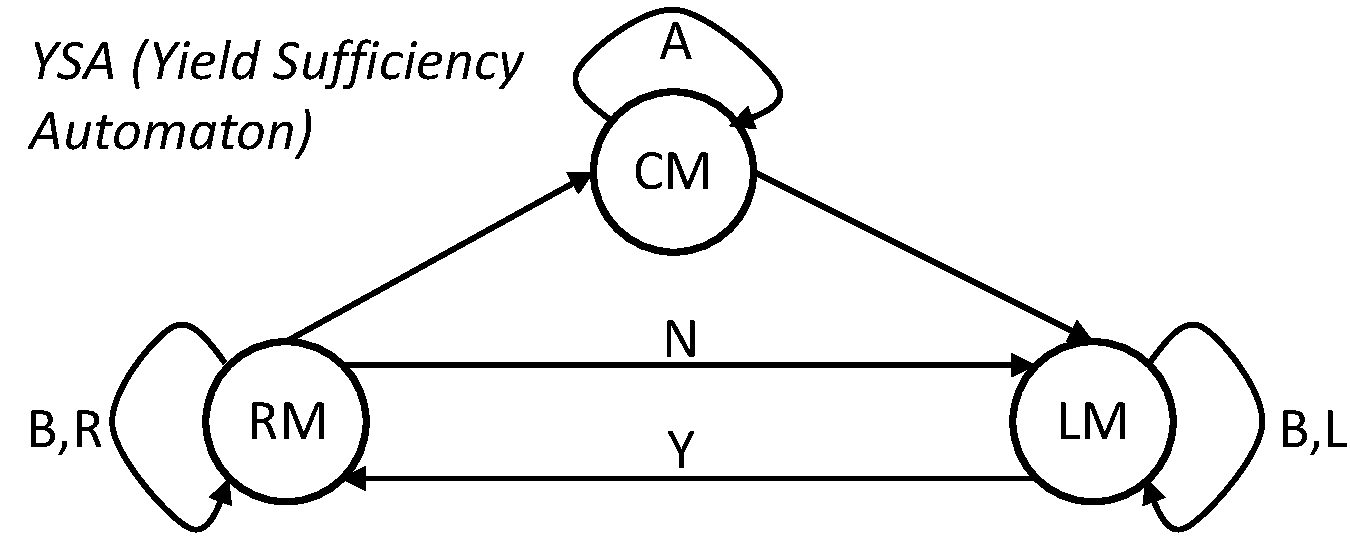
\includegraphics[scale=0.35]{YieldTypeCheckingAutomaton.pdf}
\caption{Specification for yield sufficiency}
\label{fig:YieldTypeCheckingAutomaton}
\end{figure}

\begin{figure*}
\scriptsize{
\medskip
%%%%%%%%%%%%%%%%%%%%
$
\inferrule
{
}
{\Refines;\actions \jy \skipstmt : (x, x)}
\;(\textsc{Skip})
$
\medskip
%%%%%%%%%%%%%%%%%%%%
$
\inferrule
{
}
{\Refines;\actions \jy \assert{\locExpr} : (x, x)}
\;(\textsc{Assert})
$
\medskip
%%%%%%%%%%%%%%%%%%%%
$
\inferrule
{
}
{\Refines;\actions \jy \yield{e,\lins} : (x, \RM)}
\;(\textsc{Yield})
$
\medskip
%%%%%%%%%%%%%%%%%%%%
$
\inferrule
{
P \not \in \dom(\Refines)
}
{\Refines;\actions \jy \call{P} : (x, \RM)}
\;(\textsc{Call})
$
\medskip
%%%%%%%%%%%%%%%%%%%%
$
\inferrule
{
P \in \dom(\Refines) \\ \actions(\Refines(P)) = (\rho, \alpha, B)
}
{\Refines;\actions \jy \call{P} : (x, x)}
\;(\textsc{BothMover})
$
\medskip
%%%%%%%%%%%%%%%%%%%%
$
\inferrule
{
P \in \dom(\Refines) \\ \actions(\Refines(P)) = (\rho, \alpha, R)
}
{\Refines;\actions \jy \call{P} : (\RM, \RM)}
\;(\textsc{RightMover})
$
\medskip
%%%%%%%%%%%%%%%%%%%%
$
\inferrule
{
P \in \dom(\Refines) \\ \actions(\Refines(P)) = (\rho, \alpha, L)
}
{\Refines;\actions \jy \call{P} : (x, \LM)}
\;(\textsc{LeftMover})
$
\medskip
%%%%%%%%%%%%%%%%%%%%
$
\inferrule
{
P \in \dom(\Refines) \\ \actions(\Refines(P)) = (\rho, \alpha, N)
}
{\Refines;\actions \jy \call{P} : (\RM, \LM)}
\;(\textsc{NonMover})
$
\medskip
%%%%%%%%%%%%%%%%%%%%
$
\inferrule
{
}
{\Refines;\actions \jy \async{P} : (x, \LM)}
\;(\textsc{Async})
$
\medskip
%%%%%%%%%%%%%%%%%%%%
$
\inferrule
{
x \in \{\RM,\CM\}
}
{\Refines;\actions \jy \ablock{e,\lins}{s} : (x, \CM)}
\;(\textsc{Ablock})
$
\medskip
%%%%%%%%%%%%%%%%%%%%
$
\inferrule
{
\Refines;\actions \jy \StmtStack : (x, y) \\ \Refines;\actions \jy s : (y, z)
}
{\Refines;\actions \jy \StmtStack;s : (x, z)}
\;(\textsc{Seq})
$
\medskip
%%%%%%%%%%%%%%%%%%%%
$
\inferrule
{
\Refines;\actions \jy s_1 : (x, y) \\ \Refines;\actions \jy s_2 : (x, y)
}
{\Refines;\actions \jy \ite{\locExpr}{s_1}{s_2} : (x, y)}
\;(\textsc{Ite})
$
\medskip
%%%%%%%%%%%%%%%%%%%%
$
\inferrule
{
\Refines;\actions \jy s : (x, x)
}
{\Refines;\actions \jy \while{e,\alpha}{\locExpr}{s} : (x, x)}
\;(\textsc{While})
$
\medskip
%%%%%%%%%%%%%%%%%%%%
$
\inferrule
{
\procs(P) = (\phi, \mods, \psi, \stmt) \\
\Refines;\actions \jy \stmt : (x, y)
}
{
\Refines;\actions \jy P
}
\;(\textsc{Procedure})
$
\medskip
%%%%%%%%%%%%%%%%%%%%
$
\inferrule
{
\Refines;\actions \jy \StmtStack : (x,y)
}
{
\Refines;\actions \jy (\varsL,\StmtStack) : (x,y)
}
\;(\textsc{Stack})
$
\medskip
%%%%%%%%%%%%%%%%%%%%
$
\inferrule
{
T = (\varsTL, (\varsL, \StmtStack)) \\
\Refines;\actions \jy (\varsL, \StmtStack) : (x, y)
}
{
\Refines;\actions \jy T
}
\;(\textsc{Thread})
$
\medskip
%%%%%%%%%%%%%%%%%%%%
$
\inferrule
{
\forall P \in \ProcName \setminus \dom(\Refines).\ \Refines;\actions \jy P \\\\
\forall 1 \le i \le n.\ \Refines;\actions \jy T_i
}
{
\Refines \jy (\procs, \actions, \ProcLins, \varsG, T_1 \ldots T_n)
}
\;(\textsc{Program})
$
\medskip
%%%%%%%%%%%%%%%%%%%%
}
\caption{Yield sufficiency rules}
\label{fig:yield-sufficiency}
\end{figure*}

\subsection{Program refinement}

\begin{figure*}
\scriptsize{
\medskip
%%%%%%%%%%%%%%%%%%%%
$
\inferrule
{
}
{\Refines;\RemovedActions \vdash \skipstmt \leadsto \skipstmt}
\;(\textsc{Skip})
$
\medskip
%%%%%%%%%%%%%%%%%%%%
$
\inferrule
{
}
{\Refines;\RemovedActions \vdash \assert{\locExpr} \leadsto \assert{\locExpr}}
\;(\textsc{Assert})
$
\medskip
%%%%%%%%%%%%%%%%%%%%
$
\inferrule
{
}
{\Refines;\RemovedActions \vdash \yield{e,\lins} \leadsto \yield{e,\lins}}
\;(\textsc{Yield})
$
\medskip
%%%%%%%%%%%%%%%%%%%%
$
\inferrule
{
A \not \in \RemovedActions
}
{\Refines;\RemovedActions \vdash \call{A} \leadsto \call{A}}
\;(\textsc{Atomic})
$
\medskip
%%%%%%%%%%%%%%%%%%%%
$
\inferrule
{
\Refines;\RemovedActions \vdash s \leadsto s'
}
{
\Refines;\RemovedActions \vdash \ablock{e,\lins}{s} \leadsto s'
}
\;(\textsc{Ablock-Elim})
$
\medskip
%%%%%%%%%%%%%%%%%%%%
$
\inferrule
{
\Refines;\RemovedActions \vdash s \leadsto s'
}
{
\Refines;\RemovedActions \vdash s \leadsto \ablock{e,\lins}{s'}
}
\;(\textsc{Ablock-Intro})
$
\medskip
%%%%%%%%%%%%%%%%%%%%
$
\inferrule
{
P \in \dom(\Refines)
}
{
\Refines;\RemovedActions \vdash \call{P} \leadsto \call{\Refines(P)}
}
\;(\textsc{Proc1})
$
\medskip
%%%%%%%%%%%%%%%%%%%%
$
\inferrule
{
P \not\in \dom(\Refines)
}
{
\Refines;\RemovedActions \vdash \call{P} \leadsto \call{P}
}
\;(\textsc{Proc2})
$
\medskip
%%%%%%%%%%%%%%%%%%%%
$
\inferrule
{
}
{
\Refines;\RemovedActions \vdash \async{P} \leadsto \async{P}
}
\;(\textsc{Async})
$
\medskip
%%%%%%%%%%%%%%%%%%%%
$
\inferrule
{
\Refines;\RemovedActions \vdash \StmtStack \leadsto \StmtStack'
}
{
\Refines;\RemovedActions \vdash (\varsL,\StmtStack) \leadsto (\varsL,\StmtStack')
}
\;(\textsc{Stack})
$
\medskip
%%%%%%%%%%%%%%%%%%%%
$
\inferrule
{
\Refines;\RemovedActions \vdash \StmtStack \leadsto \StmtStack' \\
\Refines;\RemovedActions \vdash \stmt \leadsto \stmt'
}
{
\Refines;\RemovedActions \vdash \StmtStack;\stmt \leadsto \StmtStack';\stmt'
}
\;(\textsc{Seq})
$
\medskip
%%%%%%%%%%%%%%%%%%%%
$
\inferrule
{
\Refines;\RemovedActions \vdash s_1 \leadsto s_1' \\
\Refines;\RemovedActions \vdash s_2 \leadsto s_2'
}
{
\Refines;\RemovedActions \vdash \ite{\locExpr}{s_1}{s_2} \leadsto \ite{\locExpr}{s_1'}{s_2'}
}
\;(\textsc{Ite})
$
\medskip
%%%%%%%%%%%%%%%%%%%%
$
\inferrule
{
\Refines;\RemovedActions \vdash s \leadsto s'
}
{
\Refines;\RemovedActions \vdash \while{e,\alpha}{\locExpr}{s} \leadsto \while{e,\alpha}{\locExpr}{s'}
}
\;(\textsc{While})
$
\medskip
%%%%%%%%%%%%%%%%%%%%
$
\inferrule
{
\Refines;\RemovedActions \vdash \stmt \leadsto \stmt'
}
{
\Refines;\RemovedActions \vdash (\phi,\mods,\psi,\stmt) \leadsto (\phi',\mods',\psi',\stmt')
}
\;(\textsc{Procedure})
$
\medskip
%%%%%%%%%%%%%%%%%%%%
$
\inferrule
{
\accessVars(\rho) \cap \Local = \emptyset \\
\alpha = ((\exists \mathit{old}(\Local), \Local.\ \alpha) \wedge \Same(\Local)) \\
}
{
\Refines;\RemovedActions \vdash (\rho,\alpha,m) \leadsto (\rho,\alpha,m)
}
\;(\textsc{Action})
$
\medskip
%%%%%%%%%%%%%%%%%%%%
$
\inferrule
{
\Refines;\RemovedActions \vdash \StmtStack \leadsto \StmtStack' \\
}
{
\Refines;\RemovedActions \vdash (\varsTL, (\varsL, \StmtStack)) \leadsto (\varsTL, (\varsL, \StmtStack')) \\
}
\;(\textsc{Thread})
$
\medskip
%%%%%%%%%%%%%%%%%%%%
$
\inferrule
{
\Prog = (\procs, \actions, \ProcLins, \varsG, T_1 \ldots T_n) \\
\Prog' = (\procs', \actions', \ProcLins', \varsG, T_1' \ldots T_n') \\
\forall 1 \le i \le n.\ \Refines;\RemovedActions \vdash T_i \leadsto T_i' \\
\forall A \not\in \RemovedActions.\ \actions(A) = \actions'(A) \\
\forall A \in \range(\Refines).\ \Refines;\RemovedActions \vdash \actions(A) \leadsto \actions(A) \\
\forall P \not\in \dom(\Refines).\ \Refines;\RemovedActions \vdash \procs(P) \leadsto \procs'(P) \\
\forall P \in \dom(\Refines).\ \ProcLins(P) = \ProcLins(\Refines(P)) \\
}
{
\Refines;\RemovedActions \vdash \Prog \leadsto \Prog'
}
\;(\textsc{Program})
$
\medskip
%%%%%%%%%%%%%%%%%%%%
}
\caption{Program refinement}
\label{fig:program-refinement}
\end{figure*}

\subsection{Soundness}

\begin{theorem}
Let $\Prog$ and $\Prog'$ be two programs.
Let $\Refines \in \ProcName \pf \ActionName$ be a partial function from procedure names to action names.
Let $\RemovedActions \in 2^{\ActionName}$ be a set of action names.
Suppose the following conditions are satisfied:
\begin{enumerate}
\item
$\vdash \Prog$ and $\vdash \Prog'$ and $\Refines;\RemovedActions \vdash \Prog \leadsto \Prog'$.
\item 
All finite executions of $\Prog'$ are safe.
\item
All infinite executions of $\Prog'$ are responsive.
\item
$\CommutativitySafe(\Prog)$.
\item
$\InterferenceFree(\Prog,\Refines)$.
\item
$\Refines \jp Prog$ and $\Refines \jr Prog$ and $\Refines \jy Prog$.
\end{enumerate}
Then all finite executions of $\Prog$ are safe.
\end{theorem}

\subsection{Responsiveness}

\[
\inferrule
{
\procs;\actions;\RefinementAny;\mods \jp \FH{e \wedge \locExpr}{s}{e} \\ e \wedge \locExpr \Rightarrow f \geq 0 \\ s \preceq (old(e \wedge \locExpr) \Rightarrow \mathit{old}(f) > f)
}
{\procs;\actions;\RefinementAny;\mods \jp \FH{e}{\while{e,\alpha,f}{\locExpr}{s}}{e \wedge \neg \locExpr}}
\;(\textsc{While})
\]

